\documentclass[10pt, spanish]{article}

\usepackage[none]{hyphenat}
\usepackage[utf8]{inputenc}
\usepackage[T1]{fontenc}
\usepackage[spanish]{babel}
\usepackage{csquotes}

\usepackage{geometry}
\def\margin{20mm}
\geometry{
    a4paper,
    left=\margin,
    right=\margin,
    top=\margin,
    bottom=\margin
}

% \usepackage[sorting=none]{biblatex}
\usepackage{hyperref}

\usepackage{lmodern}
\usepackage{enumitem}
%\setenumerate{label=(\alph*),leftmargin=0.6cm}
% \setitemize{label=---,leftmargin=0.6cm}
\usepackage{amssymb}
\usepackage{mathtools}

\renewcommand*{\thefootnote}{\fnsymbol{footnote}}

% For diagrams
\usepackage{tikz}
\usetikzlibrary{arrows}

% Theorems
\usepackage{amsthm}
\usepackage{thmtools}
\newtheorem*{lema}{Lema}
\newtheorem*{obs}{Observación}
\newtheorem*{nota}{Nota}

\addto\captionsspanish{\renewcommand\proofname{Solución}}

\theoremstyle{definition}
\newtheorem*{defin}{Definición}
\newtheorem*{prop}{Proposición}
\newtheoremstyle{break}{}{}{}{}{\bfseries}{.}{.5em}{Ejercicio #2}
\theoremstyle{break}
\newtheorem{ej}{Ejercicio}

% No indentation
\setlength\parindent{0pt}
\setlength{\parskip}{0.5em}
\let\emptyset\varnothing

% Custom math commands
\newcommand{\N}{\mathbb{N}}
\newcommand{\Z}{\mathbb{Z}}
\newcommand{\Q}{\mathbb{Q}}
\newcommand{\R}{\mathbb{R}}

\renewcommand{\geq}{\geqslant}
\renewcommand{\leq}{\leqslant}

\DeclareMathSymbol{*}{\mathbin}{symbols}{"01}

\DeclareMathOperator{\im}{Im}
%\DeclareMathOperator{\ker}{Ker}
\DeclareMathOperator{\mcm}{mcm}
\DeclareMathOperator{\mcd}{mcd}

\DeclareMathOperator{\bijmap}{\ \rlap{\ensuremath{\rightarrowtail}}%
    {\ensuremath{\mkern2mu\twoheadrightarrow}}}

\newcommand{\Zp}{\mathbb{Z}_{(p)}}

\usepackage{graphicx}
\graphicspath{ {./plots/} }


\usepackage{color}
\definecolor{gray75}{gray}{0.75}
\definecolor{pycommentcol}{rgb}{0.3,0.3,0.3}     % gray
\definecolor{pystatecol}{rgb}{0,0,0.7}           % blue
\definecolor{pystringcol}{rgb}{0,0.6,0}          % green
\definecolor{pyinbuiltscol}{rgb}{0.55,0.15,0.55} % plum
\definecolor{pyspecialcol}{rgb}{0.8,0.45,0.12}   % orange
\definecolor{mygray}{gray}{0.3}
\newcommand*{\pyfontfamily}{\fontfamily{DejaVuSansMono-TLF}\selectfont}

\usepackage{listings}
\lstset{inputpath=./}
\usepackage{xcolor}


\usepackage{textgreek}
\newcommand\pythonstyle{\lstset{
        language=Python,
        literate=%esto es para que acepte acentos
        {á}{{\'a}}1
        {í}{{\'i}}1
        {é}{{\'e}}1
        {ý}{{\'y}}1
        {ú}{{\'u}}1
        {ó}{{\'o}}1
        {ě}{{\v{e}}}1
        {š}{{\v{s}}}1
        {č}{{\v{c}}}1
        {ř}{{\v{r}}}1
        {ž}{{\v{z}}}1
        {ď}{{\v{d}}}1
        {ť}{{\v{t}}}1
        {ñ}{{\~n}}1
        {ň}{{\v{n}}}1                
        {ů}{{\r{u}}}1
        {Á}{{\'A}}1
        {Í}{{\'I}}1
        {É}{{\'E}}1
        {Ý}{{\'Y}}1
        {Ú}{{\'U}}1
        {Ó}{{\'O}}1
        {Ě}{{\v{E}}}1
        {Š}{{\v{S}}}1
        {Č}{{\v{C}}}1
        {Ř}{{\v{R}}}1
        {Ž}{{\v{Z}}}1
        {Ď}{{\v{D}}}1
        {Ť}{{\v{T}}}1
        {Ň}{{\v{N}}}1                
        {ε}{{\textepsilon}}1                
        {±}{{$\pm$}}1                
        {Ů}{{\r{U}}}1,
        basicstyle=\pyfontfamily\scriptsize,
        commentstyle=\color{pycommentcol}\itshape,
        emph={self,cls,@classmethod,@property}, % Custom highlighting
        emphstyle=\color{pyspecialcol}\itshape, % Custom highlighting style
        morestring=[b]{"""},
        stringstyle=\color{pystringcol},
        keywordstyle=\color{pystatecol},        % statements
        % remove any inbuilt functions from keywords
        deletekeywords={print},
        % Switch to predefined class that contain many, but not all,
        % inbuilt functions and classes
        classoffset=1,
        % add any inbuilts, not statements
        morekeywords={print,None,TypeError},
        keywordstyle=\color{pyinbuiltscol},
        frame=leftline,
        numberstyle=\sffamily\tiny\color{mygray},
        stepnumber=1,
        numbers=left,
        numbersep=10pt,                      
        showstringspaces=false            
}}

\usepackage[labelformat=empty, labelfont={bf,it}, textfont=bf]{caption}%ponga solo el nombre en los codigos

\pythonstyle
\begin{document}
\selectfont{\Large\textbf{Geometría computacional: Práctica 1}\hfill Adrián Lattes  Grassi} \noindent\rule{17cm}{1pt}

% \lstinputlisting[linerange={1-10}, firstnumber=1]{practica1.py}

\section{Introducción}

Se ha desarrollado un código en python para estimar parcialmente el atractor de
la función logística. He hecho una implementación de los algoritmos lo más
modular posible, para evitar la repetición de código.

En la primera parte de la entrega he estimado el valor de dos conjuntos
atractores para dos valores del parámetro $r$.

En la segunda parte he estimado los valores del parámetro $r\in(3.544,4)$ tales
que las órbitas correspondientes tienen periodo 8.

% Este es un resumen de lo
% que hace cada función (también he documentado cada función debajo de su
% cabecera):
% \begin{itemize}
%     \item \texttt{logistica(r)}: Recibe el parámetro $r$ de la
%         función logística $x\mapsto rx(x-1)$ y devuelve la función
%         correspondiente. Este es un estilo de programación funcional, puesto que
%         estoy definiendo una función que devuelve otra función, útil en este
%         caso para pasar el parámetro $r$ sólo una vez y luego trabajar con la
%         función particularizada. 
%     \item \texttt{orbita(r, x0, N)}: Calcula los primeros $N$
%         valores de la órbita correspondiente al parámetro $r$ y valor inicial
%         $x_0$.   
%     \item \texttt{periodo(orb, \textepsilon)}: Estima el periodo de una
%         órbita con cierta precisión \textepsilon dados los primeros valores de
%         una órbita, calculados con la función \texttt{orbita}. Para esto
%         considera los últimos valores de la órbita (la cantidad está determinada
%         por la variable global \texttt{N\_ULT}).
%     \item \texttt{atractor(orb, \textepsilon, per)}: Estima el conjunto atractor
%         de una órbita con cierta precisión \textepsilon, dados los primeros
%         valores de la órbita. El parámetro opcional \texttt{per} sirve para
%         indicar el periodo estimado, en caso de haber sido ya calculado. Si no
%         se pasa este parámetro la función calculará el periodo.
%     \item \texttt{estimar\_errores\_atractor(orb,per)}: Dados los primeros valores
%         de una órbita y el periodo estima el error de la aproximación de la
%         órbita, teniendo en cuenta los últimos $2$*\texttt{per} valores de la
%         órbita. 
%     % \item \texttt{}
% \end{itemize}

\section{Método}

Para realizar las estimaciones de los atractores he procedido de la siguiente manera:
\begin{enumerate}
    \item He fijado el parámetro $r$ y un valor inicial $x_0$ y he calculado los
        primeros $N$ valores de la órbita (ver función \texttt{orbita}):
        \[\forall n\in\{1,\ldots,N-1\}:\ x_n := rx_{n-1}(1-x_{n-1}).\] 
    \item Con estos valores y fijada una tolerancia $\varepsilon$ he estimado el
        periodo de la órbita, teniendo en cuenta posibles periodos $p\in\left\{
        1,\ldots, \texttt{N\_ULT}/2 \right\} $ y
        restando los últimos valores de la órbita (ver función
        \texttt{periodo}). Es decir, he determinado que la órbita tiene periodo
        $p$ si
        \[\forall j = \{1, \ldots, p\}:\ \left| x_{N-1-j}-x_{N-1-j-p} \right| <\varepsilon.\]
    \item Habiendo estimado el periodo de la órbita es fácil obtener la
        estimación del conjunto atractor: es suficiente con considerar los
        últimos $p$ valores de la sección inicial de la órbita, donde $p$ es el
        periodo (ver función \texttt{atractor}). Para estimar el error de estos puntos de la órbita se
        consideran los últimos $2*p$ valores y se resta cada uno con su
        correspondiente (ver funciones \texttt{estimar\_errores\_atractor} y
        \texttt{estimar\_error\_atractor}):
        \[e_{x_{N-1-j}}:=\left|x_{N-1-j}-x_{N-1-j-p}\right|.\]
\end{enumerate}

Para estimar los valores de $r\in(3.544, 4)$ correspondientes a las órbitas de periodo 8 he
procedido como sigue:
\begin{enumerate}
    \item He considerado $M$ puntos equidistantes en el intervalo $(3.544,4)$,
        separados entre sí por la distancia $\delta = \frac{4-3.544}{M-1}$. Para
        esto he utilizado la función \texttt{linspace} de \textit{numpy}.
    \item Para cada uno de estos valores de $r$ he calculado el periodo y si
        este periodo corresponde con el buscado (8) también conjunto atractor el
        cojunto atractor correspondiente (ver función
        \texttt{atractores\_con\_periodo}).
    \item El error estimado para los valores de $r$ obtenidos se corresponde con
        el valor $\delta$.
\end{enumerate} 

\section{Resultados}

En el primer apartado he estimado los conjuntos atractores para dos valores de
$r$, con $x_0=0.1$, $\varepsilon = 10^{-4}$ y $N=100$:
\begin{enumerate}
    \item Para $r_1=3.0241$ he obtenido una estimación del periodo $p=2$ y los
        siguientes valores del conjunto atractor:
        \begin{itemize}
            \item $x_{N-1}=0.613772835379854 \pm5.655200368437363*10^{-6}$ 
            \item $x_{N-2}=0.7168802691693898 \pm8.218621085354094*10^{-6}$ 
        \end{itemize}
    \item Para $r_2=3.4657$ he obtenido una estimación del periodo $p=4$ y los
        siguientes valores del conjunto atractor:
        \begin{itemize}
            \item $x_{N-1} = 0.4069223551243272 \pm4.0606841750223666*10^{-7}$
            \item $x_{N-2} = 0.4742289921180187 \pm1.7414951214433927*10^{-7}$
            \item $x_{N-3} = 0.8364000883509567 \pm2.6993256668772503*10^{-7}$
            \item $x_{N-4} = 0.8641233457379652 \pm1.0695121777093419*10^{-7}$
        \end{itemize}
\end{enumerate}

Estas son las gráficas correspondientes a las órbitas de estos valores de $r$.
También he dibujado una gráfica con estimaciones del conjunto atractor para
valores de $r$ en el intervalo $(2.95, 3.544)$.

\begin{center}
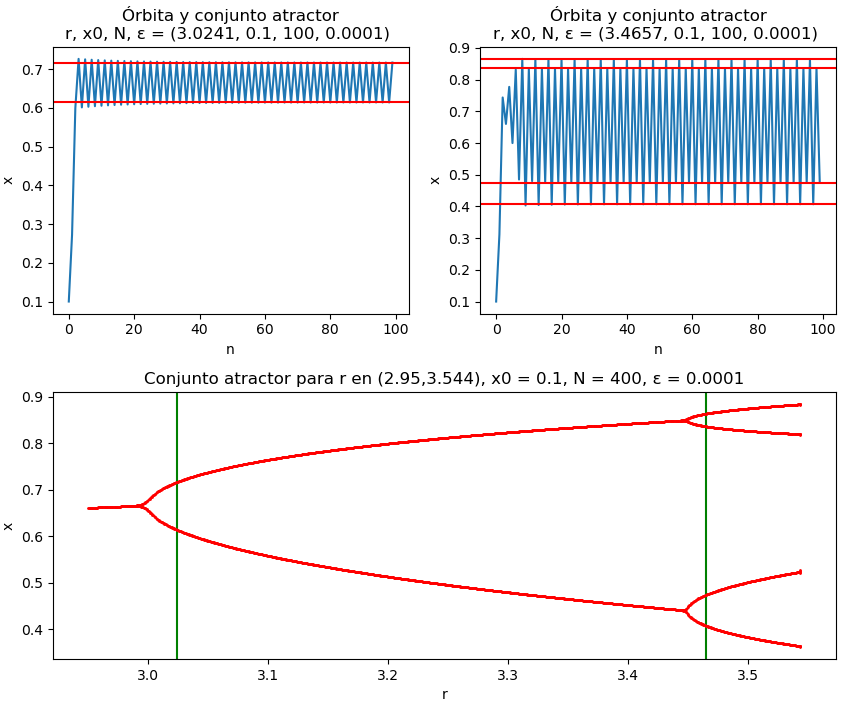
\includegraphics[width=8.5cm]{plot01}
\end{center}

Para la segunda estimación, con los valores $M=1000$, $x_0=0.5$ y
$\varepsilon=10^{-5}$ he obtenido 44 valores de $r$ con periodo $8$. El error de
estimación es $\delta = \frac{4-3.544}{1000-1}=0.000456456$. Estos son
algunos ejemplos:
\begin{itemize}
    \item $r = 3.5444564564564565\pm \delta$ es el valor más pequeño.
    \item $r= 3.5636276276276275\pm\delta$ es el valor más grande de la zona en
        la que se aprecia \textit{continuidad}.
    \item $r=3.6622222222222223\pm\delta$ es un valor que está
        visiblemente aislado de los demás.
\end{itemize}

\begin{center}
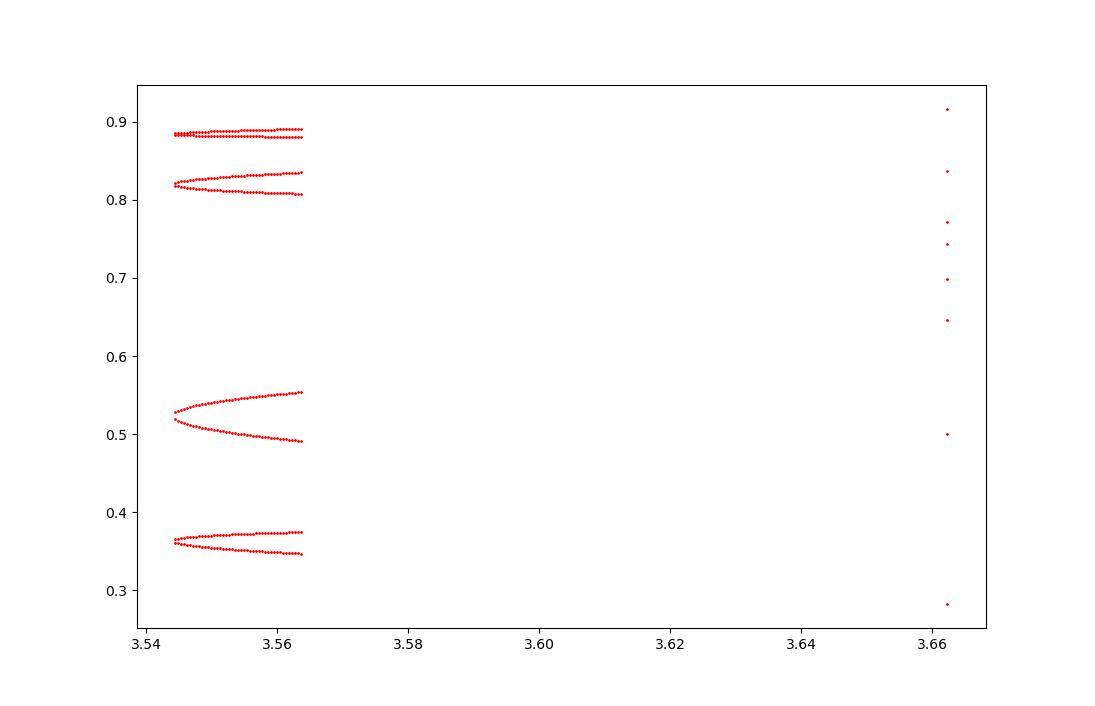
\includegraphics[width=10cm]{plot02}
\end{center}

\section{Código}

Este es el código con el que he realizado las estimaciones y las gráficas.
También está adjunto en la entrega y disponible en el repositorio git en el
siguiente enlace: \href{https://www.github.com/haztecaso/gcomp}{github.com/haztecaso/gcomp}.

% \lstinputlisting[linerange={1-10}, firstnumber=1]{practica1.py}
\lstinputlisting[linerange={4-236}, firstnumber=4]{practica1.py}

\end{document}
